\documentclass{standalone}
\usepackage{tikz}
\usetikzlibrary{patterns, positioning}
\usepackage[sfdefault]{ClearSans} %% option 'sfdefault' activates Clear Sans as the default text font
\usepackage[T1]{fontenc}

\begin{document}
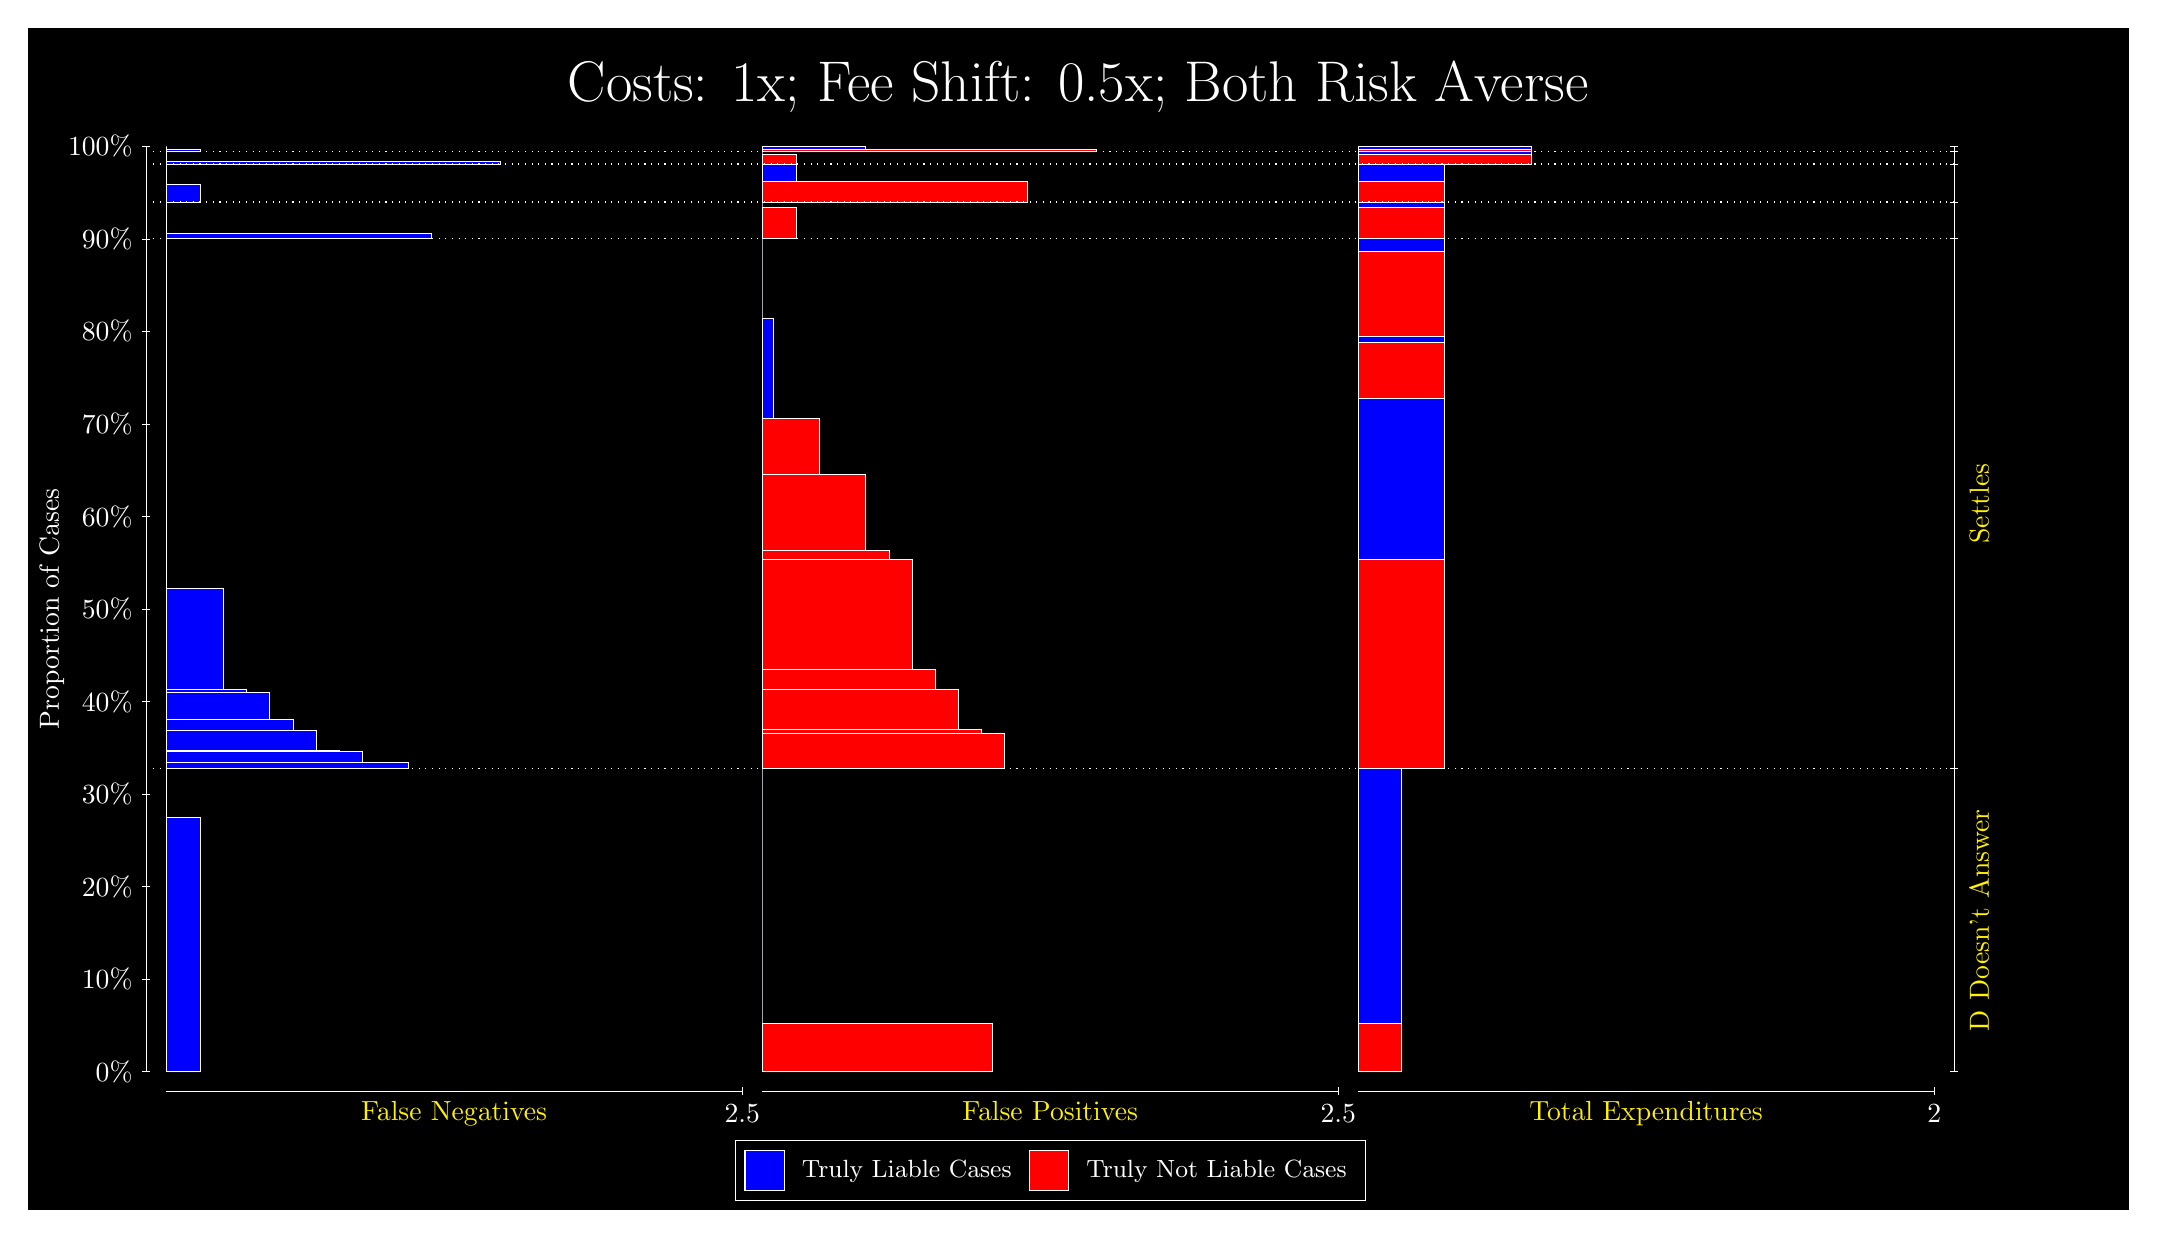
\begin{tikzpicture}
\draw[fill=black] (0,0) rectangle (26.667,15);
\draw[text=white] (0,13.5) rectangle (26.667,15) node[midway] {\huge Costs: 1x; Fee Shift: 0.5x; Both Risk Averse};
\draw[white, very thin] (1.5,1.75) -- (1.5,13.5);
\node[rotate=90, text=white, anchor=center] at (0.3, 7.625) {Proportion of Cases};
\draw[white, very thin] (1.45,1.75) -- (1.55,1.75);
\node[text=white, anchor=east] at (1.45, 1.75) {0\%};
\draw[white, very thin] (1.45,2.925) -- (1.55,2.925);
\node[text=white, anchor=east] at (1.45, 2.925) {10\%};
\draw[white, very thin] (1.45,4.1) -- (1.55,4.1);
\node[text=white, anchor=east] at (1.45, 4.1) {20\%};
\draw[white, very thin] (1.45,5.275) -- (1.55,5.275);
\node[text=white, anchor=east] at (1.45, 5.275) {30\%};
\draw[white, very thin] (1.45,6.45) -- (1.55,6.45);
\node[text=white, anchor=east] at (1.45, 6.45) {40\%};
\draw[white, very thin] (1.45,7.625) -- (1.55,7.625);
\node[text=white, anchor=east] at (1.45, 7.625) {50\%};
\draw[white, very thin] (1.45,8.8) -- (1.55,8.8);
\node[text=white, anchor=east] at (1.45, 8.8) {60\%};
\draw[white, very thin] (1.45,9.975) -- (1.55,9.975);
\node[text=white, anchor=east] at (1.45, 9.975) {70\%};
\draw[white, very thin] (1.45,11.15) -- (1.55,11.15);
\node[text=white, anchor=east] at (1.45, 11.15) {80\%};
\draw[white, very thin] (1.45,12.325) -- (1.55,12.325);
\node[text=white, anchor=east] at (1.45, 12.325) {90\%};
\draw[white, very thin] (1.45,13.5) -- (1.55,13.5);
\node[text=white, anchor=east] at (1.45, 13.5) {100\%};

\draw[white, very thin] (24.457,1.75) -- (24.457,13.5);
\draw[white, very thin] (24.407,1.75) -- (24.507,1.75);
\node[anchor=west] at (24.407, 1.75) {};
\draw[white, very thin] (24.407,5.596) -- (24.507,5.596);
\node[anchor=west] at (24.407, 5.596) {};
\draw[white, very thin] (24.407,12.33) -- (24.507,12.33);
\node[anchor=west] at (24.407, 12.33) {};
\draw[white, very thin] (24.407,12.793) -- (24.507,12.793);
\node[anchor=west] at (24.407, 12.793) {};
\draw[white, very thin] (24.407,13.276) -- (24.507,13.276);
\node[anchor=west] at (24.407, 13.276) {};
\draw[white, very thin] (24.407,13.431) -- (24.507,13.431);
\node[anchor=west] at (24.407, 13.431) {};
\draw[white, very thin] (24.407,13.5) -- (24.507,13.5);
\node[anchor=west] at (24.407, 13.5) {};

\draw[white, very thin, fill=blue] (1.75,1.75) rectangle (2.1891,4.983);
\draw[white, very thin, fill=red] (1.75,4.983) rectangle (1.75,5.596);
\draw[white, very thin, fill=blue] (1.75,5.596) rectangle (4.8239,5.6749);
\draw[white, very thin, fill=blue] (1.75,5.6749) rectangle (4.2384,5.814);
\draw[white, very thin, fill=blue] (1.75,5.814) rectangle (3.9457,5.8321);
\draw[white, very thin, fill=blue] (1.75,5.8321) rectangle (3.6529,6.0861);
\draw[white, very thin, fill=blue] (1.75,6.0861) rectangle (3.3602,6.2204);
\draw[white, very thin, fill=blue] (1.75,6.2204) rectangle (3.0674,6.5612);
\draw[white, very thin, fill=blue] (1.75,6.5612) rectangle (2.7746,6.6099);
\draw[white, very thin, fill=blue] (1.75,6.6099) rectangle (2.4819,7.8809);
\draw[white, very thin, fill=red] (1.75,7.8809) rectangle (1.75,12.33);
\draw[white, very thin, fill=blue] (1.75,12.33) rectangle (5.1167,12.398);
\draw[white, very thin, fill=red] (1.75,12.398) rectangle (1.75,12.793);
\draw[white, very thin, fill=blue] (1.75,12.793) rectangle (2.1891,13.014);
\draw[white, very thin, fill=red] (1.75,13.014) rectangle (1.75,13.276);
\draw[white, very thin, fill=blue] (1.75,13.276) rectangle (5.9949,13.31);
\draw[white, very thin, fill=red] (1.75,13.31) rectangle (1.75,13.431);
\draw[white, very thin, fill=blue] (1.75,13.431) rectangle (2.1891,13.467);
\draw[white, very thin, fill=red] (1.75,13.467) rectangle (1.75,13.5);
\draw[white, very thin, fill=red] (9.3189,1.75) rectangle (12.246,2.363);
\draw[white, very thin, fill=blue] (9.3189,2.363) rectangle (9.3189,5.596);
\draw[white, very thin, fill=red] (9.3189,5.596) rectangle (12.393,6.0453);
\draw[white, very thin, fill=red] (9.3189,6.0453) rectangle (12.1,6.0979);
\draw[white, very thin, fill=red] (9.3189,6.0979) rectangle (11.807,6.6061);
\draw[white, very thin, fill=red] (9.3189,6.6061) rectangle (11.515,6.8564);
\draw[white, very thin, fill=red] (9.3189,6.8564) rectangle (11.222,8.255);
\draw[white, very thin, fill=red] (9.3189,8.255) rectangle (10.929,8.3726);
\draw[white, very thin, fill=red] (9.3189,8.3726) rectangle (10.636,9.3365);
\draw[white, very thin, fill=red] (9.3189,9.3365) rectangle (10.051,10.045);
\draw[white, very thin, fill=blue] (9.3189,10.045) rectangle (9.4652,11.317);
\draw[white, very thin, fill=blue] (9.3189,11.317) rectangle (9.3189,12.33);
\draw[white, very thin, fill=red] (9.3189,12.33) rectangle (9.758,12.726);
\draw[white, very thin, fill=blue] (9.3189,12.726) rectangle (9.3189,12.793);
\draw[white, very thin, fill=red] (9.3189,12.793) rectangle (12.686,13.056);
\draw[white, very thin, fill=blue] (9.3189,13.056) rectangle (9.758,13.276);
\draw[white, very thin, fill=red] (9.3189,13.276) rectangle (9.758,13.397);
\draw[white, very thin, fill=blue] (9.3189,13.397) rectangle (9.3189,13.431);
\draw[white, very thin, fill=red] (9.3189,13.431) rectangle (13.564,13.463);
\draw[white, very thin, fill=blue] (9.3189,13.463) rectangle (10.636,13.5);
\draw[white, very thin, fill=red] (16.888,1.75) rectangle (17.437,2.363);
\draw[white, very thin, fill=blue] (16.888,2.363) rectangle (17.437,5.596);
\draw[white, very thin, fill=red] (16.888,5.596) rectangle (17.986,8.255);
\draw[white, very thin, fill=blue] (16.888,8.255) rectangle (17.986,10.304);
\draw[white, very thin, fill=red] (16.888,10.304) rectangle (17.986,11.013);
\draw[white, very thin, fill=blue] (16.888,11.013) rectangle (17.986,11.092);
\draw[white, very thin, fill=red] (16.888,11.092) rectangle (17.986,12.173);
\draw[white, very thin, fill=blue] (16.888,12.173) rectangle (17.986,12.33);
\draw[white, very thin, fill=red] (16.888,12.33) rectangle (17.986,12.726);
\draw[white, very thin, fill=blue] (16.888,12.726) rectangle (17.986,12.793);
\draw[white, very thin, fill=red] (16.888,12.793) rectangle (17.986,13.056);
\draw[white, very thin, fill=blue] (16.888,13.056) rectangle (17.986,13.276);
\draw[white, very thin, fill=red] (16.888,13.276) rectangle (19.083,13.397);
\draw[white, very thin, fill=blue] (16.888,13.397) rectangle (19.083,13.431);
\draw[white, very thin, fill=red] (16.888,13.431) rectangle (19.083,13.463);
\draw[white, very thin, fill=blue] (16.888,13.463) rectangle (19.083,13.5);
\draw[white, dotted] (1.5,5.596) -- (24.457,5.596);
\draw[white, dotted] (1.5,12.33) -- (24.457,12.33);
\draw[white, dotted] (1.5,12.793) -- (24.457,12.793);
\draw[white, dotted] (1.5,13.276) -- (24.457,13.276);
\draw[white, dotted] (1.5,13.431) -- (24.457,13.431);
\draw[white, very thin] (1.75,1.5) -- (9.0689,1.5);
\node[text=yellow, anchor=north] at (5.4094, 1.5) {False Negatives};
\draw[white, very thin] (9.0689,1.45) -- (9.0689,1.55);
\node[text=white, anchor=north] at (9.0689, 1.45) {2.5};

\draw[white, very thin] (9.3189,1.5) -- (16.638,1.5);
\node[text=yellow, anchor=north] at (12.978, 1.5) {False Positives};
\draw[white, very thin] (16.638,1.45) -- (16.638,1.55);
\node[text=white, anchor=north] at (16.638, 1.45) {2.5};

\draw[white, very thin] (16.888,1.5) -- (24.207,1.5);
\node[text=yellow, anchor=north] at (20.547, 1.5) {Total Expenditures};
\draw[white, very thin] (24.207,1.45) -- (24.207,1.55);
\node[text=white, anchor=north] at (24.207, 1.45) {2};

\node[text=yellow, centered, rotate=90] at (24.777, 3.673) {D Doesn't Answer};
\node[text=yellow, centered, rotate=90] at (24.777, 8.9632) {Settles};





\draw (12.978300999999998,1.5) node[draw=none] (baseCoordinate) {};
\begin{scope}[align=center]
        \matrix[scale=0.5, draw=white, below=0.5cm of baseCoordinate, nodes={draw}, column sep=0.1cm]{
            \node[rectangle, draw, minimum width=0.5cm, minimum height=0.5cm, fill=blue] {}; &
            \node[draw=none, font=\small, text=white] (B) {Truly Liable Cases}; &
            \node[rectangle, draw, minimum width=0.5cm, minimum height=0.5cm, fill=red] {}; &
            \node[draw=none, font=\small, text=white] (B) {Truly Not Liable Cases}; \\
            };
\end{scope}

\end{tikzpicture}
\end{document}